% !Mode:: "TeX:UTF-8"

%%% Local Variables:
%%% mode: latex
%%% TeX-master: t
%%% End:

% 学习排序知识库补全
\chapter{基于学习排序模型的知识库补全}
\label{cha:kbc-rank}

\section{问题引入}
当前的知识库基于打分模型进行知识库补全有很大不足。一是知识库中正负实体对比例差别很大,对于每个在知识库中实际存在的三元组正实例,可能有成千上万条不存在的三元组负实例相对应,如三元组(北京师范大学,位于,中国)这个三元组在知识库中实际存在,是一条正实例,而(北京师范大学,位于,美国)和(北京师范大学,位于,日本)等上百条负实例与之对应,如何解决正负实体对不匹配的问题很关键,正负实体对比例悬殊,关系预测中仅靠打分是不够的,很多基于排序的算法可以解决知识库中正负实例不匹配的问题。二是相关的方法都是通过评价三元组得分高低来预测结果的,是假设正例三元组中一个实体对之间的关系仅有一种,或者假设一个实体和关系的对应尾实体仅有一个,比如(美国,有总统,?)这个三元组中,尾实体通常被假设只有一个正确结果,而在现实的知识库中存在一对多的关系如:(美国,有总统,川普)和(美国,有总统,奥巴马)在知识库中都是实际存在的,并且通常来说,我们希望美国,有总统,川普)这个三元组比(美国,有总统,奥巴马)排序更高,这就需要我们不仅仅考虑实体对的得分问题,还要研究实体对相对排序情况,保证正实体对排序总在负实体对之前。而当前一些知识库补全算法并未考虑候选实体对的顺序对预测结果的影响,也不关注候选实体的秩序关系,而基于学习排序的算法可以解决候选实体的秩序关系。

本部分研究基于抽取知识库中的关系路径特征进行模型预测。模型预测主要分为两种方法:
分类模型和排序模型。传统的基于逻辑回归的分类算法对正负实体对进行分类模型学习,
利用二分类算法学习正负实体对的得分,依据得分大小将正负实体对进行划分,从而进行关系预测。
排序模型通过构建排序算法,对一组正负实体对进行学习排序,通过学习实体对的秩序排名,期望能将
正实体对排在负实体对之前,这样既可获得比传统分类回归算法更好的结果。本研究构建了基于树排序方法的
知识库补全算法和基于神经网络排序的知识库补全算法。

本研究构建了一种新的知识库补全的模型。其知识库补全的技术关键点在于:
(1)给定一个输入关系,将输入关系切分为训练集(包括验证集)和测试集;
(2)对于训练集和测试集中的正实体对基于局部封闭世界的假设,生成对应比例的负实体对;
(3)将正负实体对构成的集合在由知识库构成的图中抽取特征,
基于随机游走的算法抽取从头实体对到尾实体对的路径类型作为关系预测的特征;
(4)构建学习排序模型,将生成的正负实体对进行模型训练,并将训练获得的模型为新的关系特征提供预测;
(5)基于MAP和MRR进行模型评价,改进模型的参数,更新模型获得更好的预测效果。

考虑到结合关系路径和结合实体属性特征进行知识库补全算法的实现难度较大,本部分研究仅仅使用了关系路径特征作为知识库补全特征。除此之外,本研究将为了能更好分析正负例不匹配问题对于知识库补全问题的影响,本研究只使用MAP和MRR进行模型评估,对于不同比例的正负实体对进行排序模型效果预测。

\section{提出模型}

\subsection{实体关系特征计算}
通过给定知识库中的某个r,我们获取这个关系对应的实体对集合
$$I_s=\{(h_j,t_j)|<h_j,t_j> \in KB\}$$
并对从这个知识库所有的关系和实体组成的图中抽取连接头尾实体的关系路径,
由于连接头尾实体对之间的路径数量很大,通常需要限定关系路径的长度,
并采用随机游走算法计算选择从头实体到尾实体的关系路径类型。
对于能连接从头实体到尾实体的关系路径,我们记录这个关系路径的类型,作为模型预测的特征类型。对于知识库中的每一个实体对,
我们计算实体对是否具有某些关系类型,从而获得实体对的关系路径特征向量,作为预测模型的特征向量。对于一个关系的下所有实体对,计算获得这些实体对的特征向量组成特征矩阵,从而进行下一步的模型预测。
\subsection{基于逻辑回归的补全模型}

本研究的特征计算模块采用随机游走算法抽取给定关系下的路径类型特征。对一个给定的关系下的实体对,我们需要抽取在知识库中,能在有限路径长度下,从头实体到达尾实体的路径信息。
对于如图1知识库中实体对(北京师范大学,中国),我们在知识库中可以抽取路径类型信息如:(校长-生活在)、(位于-位于)、
(有大学-位于-位于)、(校长-出生-相邻-位于)等关系路径信息,并将这些关系路径信息作为学习排序的特征。
通常,路径长度被限制在2-6跳之间,过高则关系路径太多,计算复杂度太高,而小于2跳的关系路径则使得获得关系路径类型信息太少,不能有效提供特征。

对于抽取到的关系路径特征,传统方法构建了一个分类器模型,学习每个关系和这个关系包含的实体对集合,将预测关系问题转化成一个分类预测问题,学习每个实体对具有某种关系的概率。
$$E_r=\{(h_i,t_j),y_i\}^N_{i=1} $$
表示关系r所有的实体对集合,其中$y_i\in \{0,1\}$,其中0表示负实体对,即知识库中并不是实际存在的三元组,
1表示正实体对,表示在知识库中实际存在的实体对,通过对知识库中的实体对进行分类器模型学习,
我们可以获得测试集合中实体对的打分情况。通常这个分类器采用逻辑回归算法进行模型的训练。
具体来说,对于每个关系的实体对,传统模型采用逻辑回归学习得到的关系路径特征向量$V_r$和实体属性特征向量$V_l$。
并定义了如下的逻辑回归函数,对每个关系下的实体对集合进行评价打分。
$$f(v,w)=\frac{1}{1+e^{w(V_r \oplus V_l)}}$$
其中w表示关系路径特征和实体属性特征的学习权重参数。经典论文采用对数似然函数进行最大似然估计,
并通过随机梯度下降算法学习这些模型的参数,除此之外,还考虑到模型的过拟合和参数正则化表示,本论文定义了如下的学习目标函数:
$$L_r=\frac{1}{N}\sum_{i=1}^N \{(y_ilog(f(v,w_r)) + (1-y_i)log(1-f(v,w_r))\}+\alpha ||w_r||+\beta||w_r^2||$$
其中,$L_r$表示给定关系r的目标函数,$\alpha$和$\beta$ 分别是$l_1$ 和$l_2$正则化惩罚项的权重,对于每个关系我们采用随机梯度下降算法使得整个训练集对数损失最小,同时结合$l_1$ 和$l_2$防止过拟合。最终我们可以学习得到每个关系下的关系路径特征和实体属性特征的权重。
对于学习到的模型,我们调整不同的参数和梯度下降算法改进模型的效果。


\subsection{基于学习排序的树模型}
对于\label{sec:relational}中抽取的关系路径特征,
我们需要构建基于学习排序算法的知识库补全模型进行关系训练和关系预测。
传统的路径排序算法中,当通过随机游走计算获得路径类型信息,并获得这些关系路径的值后,
再通过基于分类或者回归的算法,计算的到每个实体对的打分值。如基于逻辑回归模型的方法,
通过构建的特征向量,对每个关系中的实体对进行打分,并将打分结果通过Sigmoid函数正则化,
最终使得模型的预测结果在[0,1]之间,对于打分值越大的实体对,其具有这种关系的概率越大,反之具有这种关系的概率越小。
这种模型实质上是将打分高的实体对排在打分低的实体对之前,
表示更可能是实际存在的实体对,也可以看做是一种pointwise的实体对排序模型。
而本论文中的研究不仅仅考虑实体对的打分高低,更关注实体对之间的排序关系,
考虑一个关系下的一组实体对,其中部分实体对是正例,部分实体对是负例,在进行模型预测中,
基于实体对排序的损失函数,其目标是期望正实体对总需要排序在负实体对前面,这样就能保证在预测的候选实体对中,排在前面的实体对是正确结果,这种对一组实体对进行整体的目标函数优化可以称为listwise的排序模型。基于listwise的排序模型通常构建的目标函数是非凹函数,难以进行模型优化,通常我们也可以考虑实体对和实体对之间的关系,正实体对的排序总在负实体对之前,则我们可以认为正实体对的打分比负实体对打分应该更高,基于正负实体对pair构建的损失函数可以看做是基于pairwise构建的目标函数,这是学习排序算法中常见的模型,
很多基于支持向量机、树方法、神经网络排序算法的模型都可以基于pairwise的学习排序模型构建。

具体来说,本论文中我们采用一种基于树模型pairwise的学习排序算法进行知识库补全,除了基于树模型的学习排序,这种学习排序模型可以拓展为其他任何基于知识向量机的、基于神经网络的学习排序模型。同时,考虑到模型构建的复杂度和代码实现难度,本论文采用pointwise学习排序模型,而其他基于pointwise、listwise的学习排序模型也可以进行知识库补全预测,传统的路径排序算法也可被看做是一种简单的pointwise的学习排序模型。
本研究通过学习正负实体对之间的pairwise损失函数,
直接优化MAP训练损失函数来进行模型参数更新,从而获得更好的模型预测结果。
我们使用基于LambdaMART树模型的学习排序算法,对于一个给定的关系r,定义目标函数:
$$F(x_i|w,c)=\sum_{i=1}^K\alpha_i\pi(f_i)+\sum_{i=1}^Nl(f_i(x),f'_i(x))+\frac{C}{2}WW^T$$
其中第一项中的$\sum_{i=1}^K\alpha_i\pi(f_i)$是描述树复杂度的函数,总共有K个树进行模型训练。而第二项中$l(f_i(x),f'_i(x))$是模型的训练误差函数,
其中$f_i (x)$是每个实体对的实际分数,而$f'_i(x)$是通过模型学习得到的预测值,共训练了N轮,
训练误差函数可以根据实际需要改变,常见的训练误差函数可以选择MAP、AUC、NDCG等不同排序指标,
通常学习排序中MAP评价指标最为常见。考虑到我们目标函数是pairwise损失函数最小化,我们也选择MAP作为训练损失函数进行模型训练。
第三部分$\frac{C}{2}WW^T$是模型的惩罚项,是防止模型在训练数据中过拟合的L2惩罚函数。

基于树模型的构建函数相比于传统的逻辑回归等分类算法,树模型有更好的模型优化能力,
通过构建单个树的分类回归模型,并将多个树模型进行叠加进行梯度下降算法,
进一步优化模型的损失函数,通过重新将模型的损失函数选择为MAP、NDCG等排序预测指标,
树模型能直接对这些指标进行预测。树模型能处理稀疏矩阵,同时能结合不同类型的关系路径特征进行模型预测。本部分选择基于学习排序的树模型进行模型构建,主要有以下考虑:(1)树模型相比于逻辑回归,更能有效的学习模型的真实分布,通过多个弱模型进行叠加改进参数,能保障树模型的损失函数下降结果更好。(2)相比于传统逻辑回归,树模型有更好的模型泛化效果,更能有效进行模型预测,相比之下逻辑回归更容易出现模型的过拟合。(3)树模型在处理稀疏向量,正负例比例差别很大的数据时,无论何种情况都有很好的模型优化性能。除此之外,本研究的学习排序模型也可以选择其他的线性的、非线性的、基于神经网络的各种模型。都能获得好的模型预测效果。

\section{模型实验}
\label{cha:exp-relational}

本研究构建了一个面向YAGO2的知识库补全实例,YAGO是一个从维基百科上抽取的、包含地理名词、WordNet等数据的知识库。而YAGO2是YAGO的一个实例,
当前YAGO2包括超过千万的实体和超过1.2亿的实体知识,我们使用了其中实体的关系型三元组共有4,484,914条、37种关系类型。
对于YAGO2知识库的实验数据的构建,我们按照37种不同的关系类型,将知识库切分为37份不同关系的实体对集合。
对于每个关系,首先基于知识库中的三元组抽取正实体对,对于每个由(头实体,尾实体)构成实体对,
基于局部封闭世界假设,使用当前关系中的其他实体随机替换生成n个对应的负实体对,其中$\frac{n}{2}$个随机替换头实体,$\frac{n}{2}$个随机替换尾实体。
生成正负实体对后,我们按照4:1的比例将这些实体对切分为训练集合和测试集合,
这样就完成了YAGO知识库中正负实体对、训练测试数据集的生成。同时,为了能研究不同比例的正负实体对下,模型预测的效果,我们设定了n的不同数值。本研究中分析了正负例三元组在比例为1:4和1:10下的模型预测效果,研究不同比例下模型的预测结果差别。

% Table generated by Excel2LaTeX from sheet 'Sheet1'
\begin{table}[htbp]
  \centering
  \caption{基于学习排序的YAGO知识库补全评价结果}
    \begin{tabular}{|l|r|r|r|r|r|r|r|r|}
    \hline
          & \multicolumn{1}{l|}{rankSFE-4} & \multicolumn{1}{l|}{rankPRA-4} & \multicolumn{1}{l|}{SFE-4} & \multicolumn{1}{l|}{PRA-4} & \multicolumn{1}{l|}{rankSFE-10} & \multicolumn{1}{l|}{rankPRA-10} & \multicolumn{1}{l|}{SFE-10} & \multicolumn{1}{l|}{PRA-10} \bigstrut\\
    \hline
    MAP   & 80.68\% & 80.06\% & 70.31\% & 69.35\% & 47.33\% & 46.91\% & 30.83\% & 31.27\% \bigstrut\\
    \hline
    MRR   & 100.00\% & 100.00\% & 97.83\% & 97.83\% & 91.95\% & 89.62\% & 90.48\% & 92.14\% \bigstrut\\
    \hline
    \end{tabular}%
  \label{tab:kbc-yago-rank}%
\end{table}%

我们计算了基于YAGO2的总体MAP和MRR进行模型评价的结果。如表\ref{tab:kbc-yago-rank}可以看到基于学习排序的知识库补全技术相比传统的路径排序算法在MAP上有很大的提升,
在正负实体对比例为1:10的情况下,
基于学习排序的算法相比传统的算法在YAGO2数据集上有近50\%的效果提升;而四种方法在MRR指标上效果相当,
基于学习排序算法的MRR并未比传统路径排序算法有显著下降。
在正负实体对比例为1:4的情况下,基于学习排序算法相比于传统的在YAGO数据集上的逻辑回归算法,
基于MAP预测的准确率提升超过10\%,效果提升近15\%。同时,对比不同比例的正负实体对分析可以发现,
当负例三元组出现较多时,对预测结果有较大的影响,正负三元组比例超过1:10时,模型预测的MAP指标不足50\%,这表明在进行学习排序模型,选择合适的正负例三元组作为预测模型的候选实体对也很重要,对于一个高效合理的模型,如何选择恰当的候选实体作为预测模型,也是知识库补全后续研究中的重要问题,本研究基于局部封闭世界假设,随机选择若干比例的候选正负实体对进行模型构建,而在后续的研究中,如何构建模型选择合适的候选正负实体对是十分必要的。

\begin{table}[htbp]
  \centering
  \caption{正负例1:10的学习排序算法部分关系MAP值}
    \begin{tabular}{|l|r|r|r|r|}
    \hline
    relation & \multicolumn{1}{l|}{PRA-10} & \multicolumn{1}{l|}{SFE-10} & \multicolumn{1}{l|}{rankPRA-10} & \multicolumn{1}{l|}{rankSFE-10} \\
    \hline
    actedIn & 0.3379  & 0.3496  & 0.6222  & 0.6252  \\
    \hline
    created & 0.2523  & 0.2532  & 0.3089  & 0.3128  \\
    \hline
    dealsWith & 0.1729  & 0.1411  & 0.1265  & 0.1572  \\
    \hline
    graduatedFrom & 0.2646  & 0.2726  & 0.5607  & 0.5726  \\
    \hline
    hasCapital & 0.5637  & 0.6014  & 0.7275  & 0.7304  \\
    \hline
    hasChild & 0.5004  & 0.5078  & 0.6674  & 0.6757  \\
    \hline
    influences & 0.2946  & 0.2932  & 0.5771  & 0.5836  \\
    \hline
    isAffiliatedTo & 0.6364  & 0.6538  & 0.7816  & 0.7840  \\
    \hline
    playsFor & 0.6538  & 0.6606  & 0.8020  & 0.8036  \\
    \hline
    wasBornIn & 0.3661  & 0.3742  & 0.6053  & 0.6070  \\
    \hline
    worksAt & 0.2343  & 0.2281  & 0.5022  & 0.5014  \\
    \hline
    wroteMusicFor & 0.3488  & 0.3621  & 0.6144  & 0.6161  \\
    \hline
    \end{tabular}%
  \label{kbc-yago-rank10}%
\end{table}%

我们详细分析了37种YAGO2中关系的MAP指标,并在表 \ref{kbc-yago-rank10}展示了部分关系在正负例为1:10的情况下的MAP值。
分析可以发现,大部分关系采用学习排序算法后,预测结果有较大的提高,而在不同的关系类型预测中,
MAP差别较大,如playFor、dealsWith和isConnectedTo等关系预测MAP有较大的提高,而在isInterestedIn等关系中关系预测提升较差。总体来说,有超过30种关系的MAP预测获得了显著的提升,只有不到5种关系MAP预测结果并未有统计上的显著提升,这说明了基于学习排序算法的知识库补全技术相比传统的分类回归打分模型对于大多数知识库预测的关系,在模型效果上有非常大的效果提升。我们进一步分析了不同export、import等关系预测中效果较差的模型,
通过分析这个模型构建中的三元组可以发现,在export和import等关系中,经常出现三元组如(China,export,Amercia),(China,export,Europe)、(America,export,China)等多重三元组,如图\ref{many2many}所示,这些类型的三元组可以看做是一种多对多的关系,在进行这类知识库补全预测模型构建中,很难利用国家和国家之间的关系路径、实体属性等信息进行模型构建,我们需要找到更好的模型预测方法,加入更多的背景知识进行知识库补全预测。

\begin{figure}[H]
\begin{center}
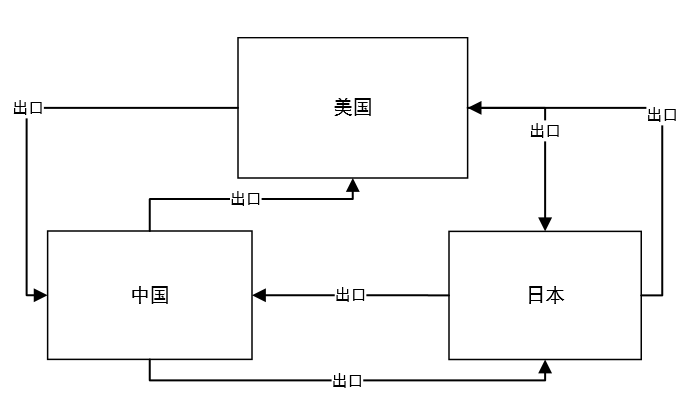
\includegraphics [width=0.6\textwidth]{many2many.PNG}
\caption{多对多实体关系的知识库}
\label{many2many}
\end{center}
\end{figure}


除了上述的1:10的知识库补全预测模型中MAP预测结果,表\ref{tab:kbc-yago-rank4}展示了在知识库补全正负例为1:4的情况下,部分关系中知识库补全MAP预测结果。
相比于1:10的正负例实体对,
基于1:4的正负例实体对能显著增加MAP预测结果的准确率,总体的平均准确率MAP值从47\%提升至80\%,这说明在选择候选实体对作为学习排序的数据时,选择实体对的比例也很关键,对于部分关系,如worksAt、dealsWith等,这些关系提升超过100\%,我们分析了相关关系下的三元组发现,这些关系下的三元组存在一对多,多对多的情况,这种情况下减少模型的候选实体对比例,能有效的提高模型的效果。通过对比不同正负比例的实体对预测情况,说明在进行知识库补全的学习排序模型构建中,如何选择候选实体对,构建合理有效的知识库补全正负实体对,也会影响知识库补全模型的结果好坏。这和很多推荐系统算法类似,
如何从百万级别的数据中选择若干候选实体对给用户推荐出来,也是具有类似的过程,通常这在推荐系统中被分为候选集生成和候选集排序两个步骤。与这种“候选-排序”两步排序算法类似,如何从上万个负实体对中选择合适的候选负实体对,组成训练模型进行排序算法的训练,是知识库补全中即为重要的一步。后续研究可以借鉴表示学习如神经网络翻译模型等实现更好的知识库补全候选实体对生成。

本部分的实验结果有如下结论:(1)基于学习排序的知识库补全算法相比于传统的逻辑回归算法,能大大提升模型预测的MAP指标,这在知识库补全算法中极为重要;(2)基于学习排序算法对于大部分关系都能产生较大的预测结果提升,而对于一些频繁出现多对多关系的正负实体对中,候选实体对选择较为困难,生成正负例三元组难以区分,如何构造有表达力的特征向量任然是一个有挑战性的工作;(3)不同正负比例的三元组预测模型效果差别很大,这表明除了选择合理有效的排序算法之外,如何构建模型,生成合理有效的候选正负实体对也是十分重要的。后续可以借鉴推荐系统中的候选集合生成算法,优化知识库补全模型中的实体对生成,也可以考虑集成表示学习中的实体向量表示,学习获得合理的候选实体对集合。

% Table generated by Excel2LaTeX from sheet 'Sheet3'
\begin{table}[htbp]
  \centering
  \caption{正负例1:4的学习排序算法部分关系MAP值}
    \begin{tabular}{|l|r|r|r|r|}
    \hline
          & \multicolumn{1}{l|}{rankSFE-4} & \multicolumn{1}{l|}{rankPRA-4} & \multicolumn{1}{l|}{SFE-4} & \multicolumn{1}{l|}{PRA-4} \bigstrut\\
    \hline
    actedIn                                                     & 0.7925  & 0.7695  & 0.7451  & 0.6941  \bigstrut\\
    \hline
    dealsWith                                                   & 0.5342  & 0.5571  & 0.4235  & 0.4073  \bigstrut\\
    \hline
    diedIn                                                      & 0.9111  & 0.9136  & 0.8231  & 0.8228  \bigstrut\\
    \hline
    graduatedFrom                                               & 0.6561  & 0.6696  & 0.4632  & 0.3980  \bigstrut\\
    \hline
    hasChild                                                    & 0.9583  & 0.9583  & 0.9167  & 0.9167  \bigstrut\\
    \hline
    hasNeighbor                                                 & 0.7663  & 0.7818  & 0.6900  & 0.7506  \bigstrut\\
    \hline
    isCitizenOf                                                 & 0.8409  & 0.8398  & 0.6500  & 0.6345  \bigstrut\\
    \hline
    isConnectedTo                                               & 0.6947  & 0.6931  & 0.3820  & 0.3595  \bigstrut\\
    \hline
    isLeaderOf                                                  & 0.9448  & 0.8499  & 0.7172  & 0.7901  \bigstrut\\
    \hline
    isLocatedIn                                                 & 0.9534  & 0.9492  & 0.8613  & 0.8564  \bigstrut\\
    \hline
    isMarriedTo                                                 & 0.8843  & 0.8752  & 0.8118  & 0.7884  \bigstrut\\
    \hline
    livesIn                                                     & 0.8080  & 0.7894  & 0.6727  & 0.6896  \bigstrut\\
    \hline
    wasBornIn                                                   & 0.9591  & 0.9560  & 0.8541  & 0.8402  \bigstrut\\
    \hline
    worksAt                                                     & 0.5053  & 0.4659  & 0.4270  & 0.3843  \bigstrut\\
    \hline
    \end{tabular}%
  \label{tab:kbc-yago-rank4}%
\end{table}%

\section{本章工作总结}
本章中,我们主要比较了基于逻辑回归分类模型和基于学习排序的树模型,通过优化知识库补全中的模型构建,我们使用基于pairwise的树排序模型,更好的提升了知识库补全中实体对之间的排序问题,将传统的基于逻辑回归的分类问题转化为基于学习排序的模型优化问题。
本研究通过对YAGO知识库进行试验发现,不同知识库补全模型中,基于排序的模型优化算法可以大幅提高正实体对在所有实体对中的秩序,从而能改变原有的知识库补全优化中仅仅对实体对进行打分的模式,能够获得更好的预测效果。对于多数关系而言,基于学习排序的树模型算法效果明显优于传统的逻辑回归分类算法。
